\documentclass{report}

\begin{document}
\chapter{Логическое проектирование реляционной модели базы данных}

\section{Нормализация отношений}

Выполнять процедуру нормализации будем над реляционной моделью 
данных, построенной один в один из ER-модели. 

На данный момент 
каждое отношение имеет следующие свойства:
\begin{itemize}
    \item в отношении нет атрибутов с одинаковым смыслом
    \item у отношения есть ключ
    \item все неключевые атрибуты функционально зависят от ключа целиком, но не от его части
    \item неключевые атрибуты нетранзитивно функционально зависят от ключей
\end{itemize} 
Чтобы получить 1НФ необходимо избавиться от неатомарных атрибутов. 
Абонент имеет неатомарный атрибут ФИО. Разделим его на три атрибута - 
фамилия, имя, отчество. Теперь все отношения в 1НФ.

Все неключевые атрибуты функционально зависят от ключа целиком и отношения
находятся в 1НФ, следовательно отношения находятся во 2 НФ. Далее, неключевые 
атрибуты нетранзитивно функционально зависят от ключей и отношения находятся
во 2НФ, следовательно отношения находятся в 3 НФ.

\section{Реляционная схема}

Для типа телефона создадим новое перечисление phone\_type =
(``Common'', ``Parallel'', ``Paired'').

\begin{longtblr}[caption={Реляционная схема базы данных}, theme = TC,]{
        colspec={|X[3]|X[3]|X[2]|X[1]|X[4]|}, row{1} = {c}, hlines,
    }
    Отношение & Атрибут & Тип & Not null & Ограничения \\
    \SetCell[r=4]{c} ATS & id & serial & + & PK \\ 
    & owner & varchar$[30]$ & - & \\
    & first number & int & + & $(0, 1'000'000'000)$ \\
    & last number & int & + & $(1, 1'000'000'000)$ \\ 
    \SetCell[r=1]{c} City ATS & id & int & + & PK-FK \\
    \SetCell[r=1]{c} Department ATS & id & int & + & PK-FK \\
    \SetCell[r=1]{c} Institution ATS & id & int & + & PK-FK \\ 
    \SetCell[r=4]{c} Base phone number & id & bigserial & + & PK \\
    & ATS & int & + & FK \\ 
    & number & int & + & $(1, 1'000'000'000)$ \\
    & address & int & + & FK \\ 
    \SetCell[r=1]{c} Payphone & id & bigint & + & PK-FK \\
    \SetCell[r=2]{c} Phone number & id & bigint & + & PK-FK \\ 
    & apartment & int & - & $>0$\\ 
    \SetCell[r=8]{c} Subsriber & id & bigserial & + & PK \\ 
    & first name & varchar$[20]$ & + & \\
    & last name & varchar$[30]$ & + & \\
    & surname & varchar$[20]$ & - & \\
    & sex & char$[1]$ & - & `m' или `f' \\
    & age & smallint & - & $(13, 131)$ \\ 
    & benefit & smallint & + & $[0, 100], default=0$ \\ 
    & debt & bigint & + & $\geq 0, default=0$ \\ 
    \SetCell[r=4]{c} Subsription & id & bigserial & + & PK \\ 
    & phone number & bigint & + & FK \\
    & subsriber & bigint & + & FK \\
    & phone type & phone\_type & + & $default=$ Common \\ 
    \SetCell[r=3]{c} Service & id & serial & + & PK \\ 
    & name & varchar$[20]$ & + & \\
    & cost & int & + & $\geq 0, default=0$ \\
    \SetCell[r=3]{c} Connection & subsription & bigserial & + & PK-FK \\ 
    & service & int & + & PK-FK \\
    & payment date  & date & + & $default=$ current date \\
    \SetCell[r=5]{c} Call log & subsriber & bigint & + & PK-FK \\ 
    & phone number & bigint & + & PK-FK \\
    & date time & timestamptz & + & PK \\
    & destination & int & + & FK \\
    & duration & int & + & $>0, default=1$ \\
    \SetCell[r=2]{c} City & id & serial & + & PK \\ 
    & name & varchar$[20]$ & + & \\ 
    \SetCell[r=3]{c} District & id & serial & + & PK \\ 
    & city & int & + & FK \\ 
    & name & varchar$[30]$ & + & \\ 
    \SetCell[r=3]{c} Street & id & serial & + & PK \\ 
    & district & int & + & FK \\ 
    & name & varchar$[30]$ & + & \\ 
    \SetCell[r=3]{c} Address & id & serial & + & PK \\ 
    & street & int & + & FK \\ 
    & house number & smallint & + & $>0$ \\ 
\end{longtblr}

\begin{figure}[!ht]
    \begin{center}
    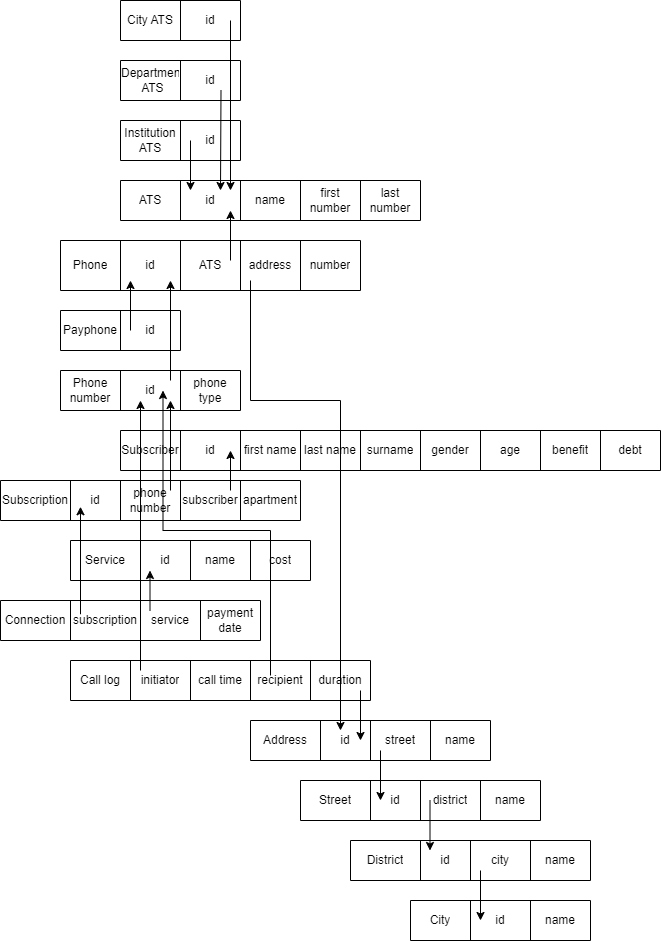
\includegraphics[height=0.9\textheight, keepaspectratio, width=\textwidth]{resources/vertical.png}
    \caption{Вертикальная диаграмма}
    \end{center}
\end{figure}

\end{document}
